\section{Cabling maps}\label{sec:cabling}

Text source of everything here: \file{docs/knowledge/wiring.md} and \file{escon/README.md}. Pin numbers
are from the maxon, Futek and Mean Well datasheets in \file{docs/reference/} and \file{escon/}.

\warn{The 230\,V side of both supplies (L, N, earth) is electrician work only. Before touching anything on
the 48\,V side: mains off, then measure the chopper pins 4--5 below 1\,V (it holds 8800\,\textmu F).}

\subsection{Power chain per tower}\label{sec:power}

\begin{figure}[H]\centering
\resizebox{\linewidth}{!}{%
\begin{tikzpicture}[
  box/.style={draw, rounded corners=2pt, align=left, font=\small, inner sep=5pt, anchor=north west},
  pwr/.style={very thick, red!70!black},
  gnd/.style={very thick, black},
  pe/.style={thick, green!50!black, dashed},
  lab/.style={font=\scriptsize, above, inner sep=2pt}]
  \newcommand{\wire}[5]{\draw[#1] ($(#2.north east)+(0,#4)$) -- node[lab]{#5} ($(#3.north west)+(0,#4)$);}
  \node[box, fill=black!4, text width=2.7cm, minimum height=2.5cm] (strip) at (0,0) {\textbf{Power strip}\\one per tower,\\own wall socket};
  \node[box, fill=red!5, text width=3.0cm, minimum height=2.5cm] (psu) at (4.6,0) {\textbf{RSP-2000-48}\\mains: L, N, earth\\DC: +V, $-$V\\CN501: e-stop};
  \node[box, fill=red!5, text width=3.6cm, minimum height=2.5cm] (chop) at (10.2,0) {\textbf{DSR 70/30 chopper}\\3 earth\\4 +V in, 5 GND in\\6 +V out, 7 GND out\\DIP switches: 55\,V};
  \node[box, text width=2.4cm, minimum height=2.5cm] (escon) at (16.6,0) {\textbf{ESCON 70/10}\\J1 +\\J1 $-$};
  \wire{pwr}{strip}{psu}{-0.8}{230\,V}
  \wire{pwr}{psu}{chop}{-0.7}{+V $\rightarrow$ 4}
  \wire{gnd}{psu}{chop}{-1.3}{$-$V $\rightarrow$ 5}
  \wire{pe}{psu}{chop}{-1.9}{earth $\rightarrow$ 3}
  \wire{pwr}{chop}{escon}{-0.9}{6 $\rightarrow$ J1+}
  \wire{gnd}{chop}{escon}{-1.5}{7 $\rightarrow$ J1$-$}
  \node[box, fill=red!5, text width=3.0cm, minimum height=1.5cm] (rs) at (4.6,-3.3) {\textbf{RS-15-24}\\+V, $-$V};
  \node[box, text width=3.6cm, minimum height=1.5cm] (amp) at (10.2,-3.3) {\textbf{Futek IAA100}\\1 +Vin, 2 GND};
  \draw[pwr] ($(strip.south)$) |- node[lab, pos=0.75]{230\,V} ($(rs.north west)+(0,-0.8)$);
  \wire{pwr}{rs}{amp}{-0.6}{+V $\rightarrow$ 1}
  \wire{gnd}{rs}{amp}{-1.1}{$-$V $\rightarrow$ 2}
\end{tikzpicture}}
\caption{Power wiring of one tower (Stanford guide pp.\,14--16, chopper and supply datasheets). Mains side: electrician only.}
\label{fig:power}
\end{figure}

\begin{itemize}
\item \textbf{One power strip per tower, each on its own wall socket.} Never plug a strip into a strip: an
RSP-2000 draws up to 50\,A inrush and about 10\,A at full load (DGUV rules).
\item The RSP-2000 has no switch: it is on whenever its mains cable is live.
\item Chopper $\rightarrow$ ESCON cable: Stanford uses 14\,AWG ($\approx$ 2\,mm$^2$). The chopper terminals take
0.14--1.5\,mm$^2$, ESCON J1 takes 0.2--2.5\,mm$^2$. Crimp blue insulated pin terminals (1.5--2.5\,mm$^2$,
pin $\approx$ 1.9\,mm; try one in the chopper first) with a crimper for insulated terminals, or use 1.5\,mm$^2$
wire with 1.5\,mm$^2$ ferrules. A ferrule crimper does not crimp pin terminals.
\item Open on tower B (electrician): earth wire supply $\rightarrow$ chopper terminal 3; cover for the
RS-15-24's open 230\,V terminals.
\end{itemize}

\subsection{ESCON 70/10 connectors}

\begin{table}[H]\centering\small
\begin{tabularx}{\linewidth}{llX}
\toprule
Connector & Pin & Use in Bump'em \\
\midrule
J1 Power & +, $-$ & 48\,V from chopper pins 6 / 7 \\
J2 Motor & 1, 2, 3 & windings 1, 2, 3: red, brown, white \\
         & 4 & cable shield: \textbf{empty} \\
J3 Hall  & 1, 2, 3 & Hall 1, 2, 3: yellow, pink, grey \\
         & 4, 5 & +5\,V Hall supply: green; GND: blue \\
J5 Digital I/O & 2 & DigIN2 = \textbf{enable} $\leftarrow$ Teensy 27/28/29/30 (yellow) \\
               & 5 & GND $\rightarrow$ ground distributor \\
               & 6 & +5\,V out: \textbf{never to a Teensy pin} \\
J6 Analog I/O  & 3, 4 & AnIN2+ / AnIN2$-$ = \textbf{setpoint} $\leftarrow$ DAC VA--VD (blue) / DAC GND (green) \\
               & 5, 6 & analog outputs, $-4$\ldots$+4$\,V: \textbf{never to a Teensy pin} \\
               & 7 & GND $\rightarrow$ ground distributor \\
J7 USB & & ESCON Studio (Windows) for configuration only \\
\bottomrule
\end{tabularx}
\caption{ESCON pins (hardware reference Tables 3-12, 3-17, 3-19). J2/J3 colours as found on module C;
check every module against this table before the first drive.}
\end{table}

\paragraph{Motor connector.} The EC 90 flat 500267 has one 8-pin Molex connector: 1 Hall 1, 2 Hall 2,
3 V\textsubscript{Hall}, 4 winding 3, 5 Hall 3, 6 Hall GND, 7 winding 1, 8 winding 2
(\file{docs/reference/maxon-500267-catalog-page.pdf}). Hall GND (blue) belongs on J3 pin 5, not on the J2
shield pin; two modules had it wrong (Sect.~\ref{sec:lessons}).

\begin{figure}[H]\centering
\begin{minipage}{0.48\linewidth}\centering
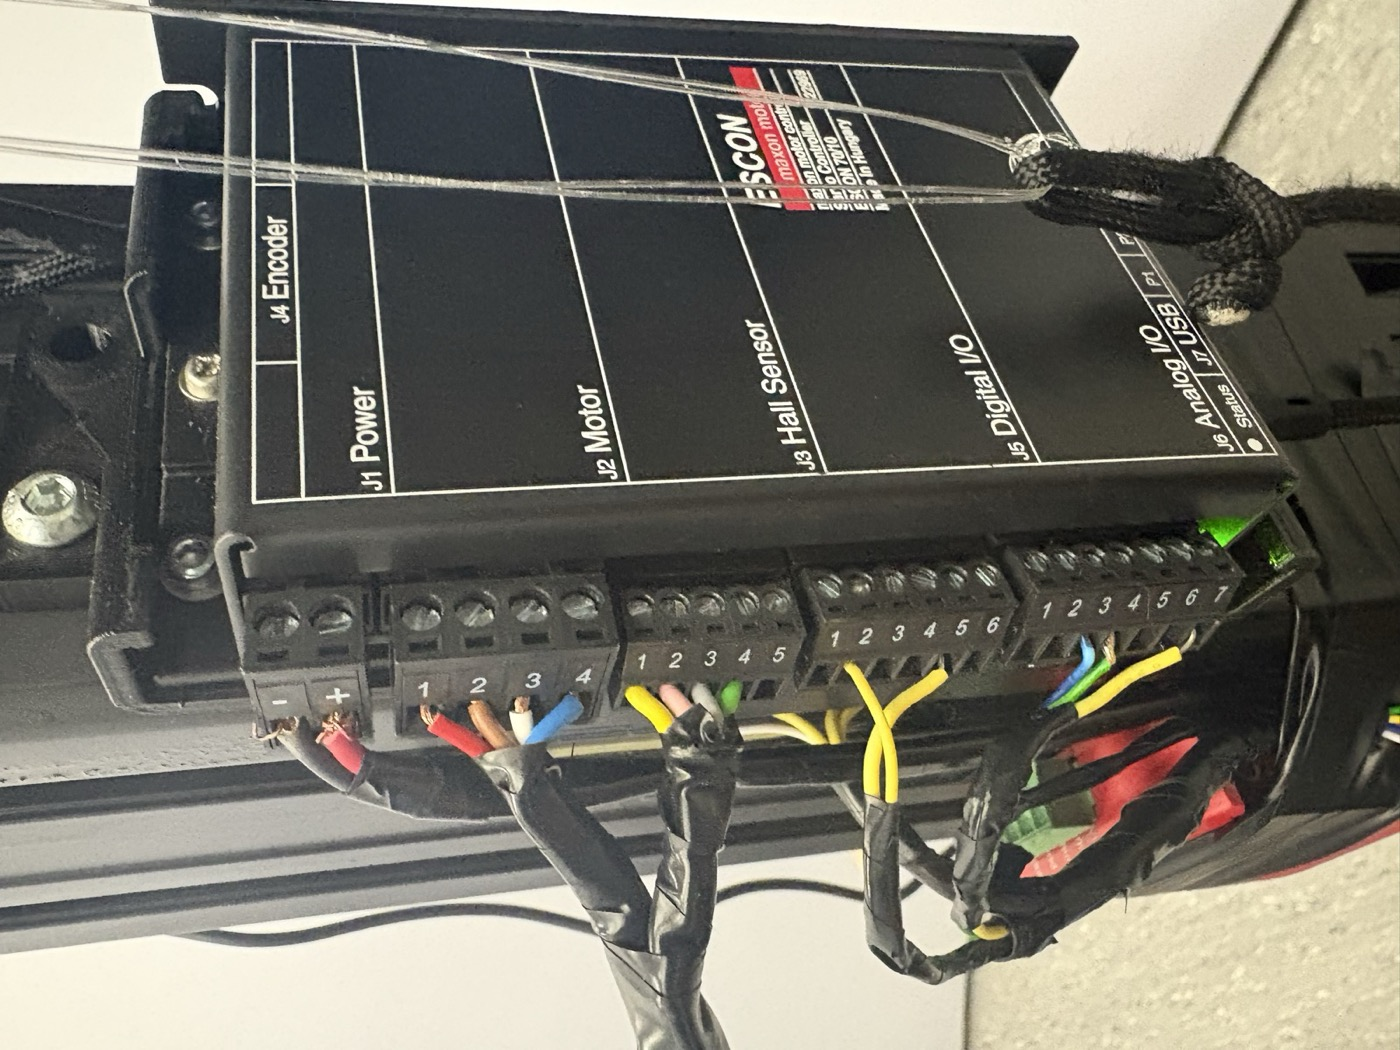
\includegraphics[width=\linewidth]{figures/2026-10-01_escon-moduleC-all-connectors.jpg}\\\small Module C, all plugs readable (before the Hall GND fix)
\end{minipage}\hfill
\begin{minipage}{0.48\linewidth}\centering
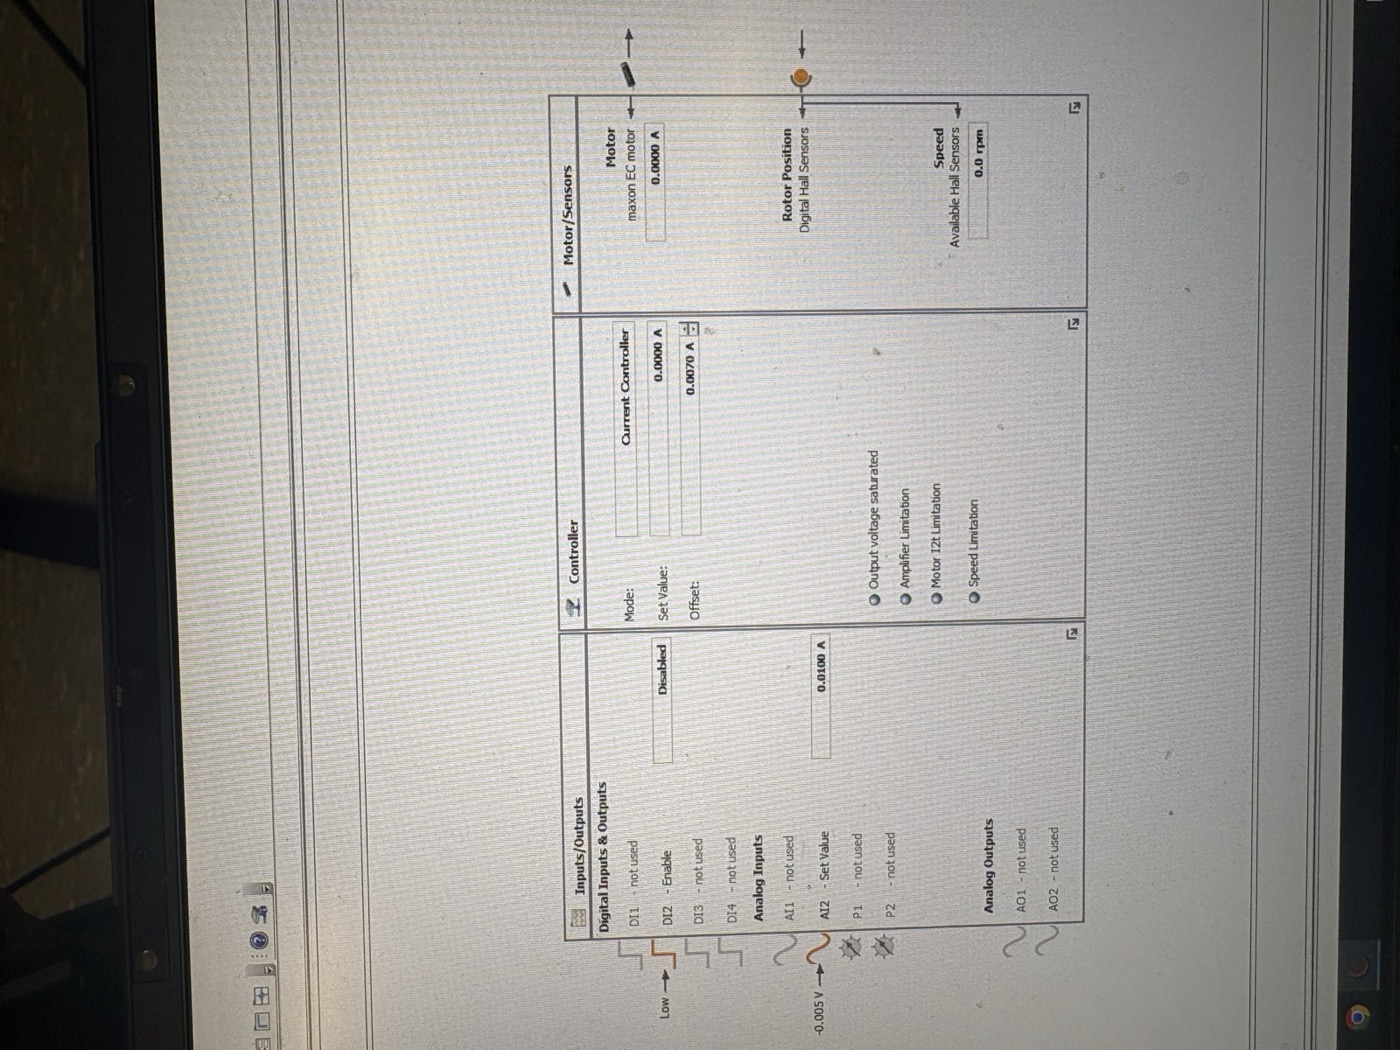
\includegraphics[width=\linewidth]{figures/2026-10-01_escon-studio-controller-monitor-moduleC.jpg}\\\small ESCON Studio controller monitor, module C
\end{minipage}
\end{figure}

\paragraph{Futek IAA100.} Power side (5-way): 1 +Vin 12.5--26\,V, 2 GND (power), 3 shunt cal (empty),
4 GND (output), 5 Vout. Sensor side (4-way): 1 +excitation, 2 +signal, 3 $-$signal,
4 $-$excitation or shield.
Vout (brown) goes to the Teensy force pin, output GND to the ground distributor.

\subsection{Control board $\leftrightarrow$ modules}

\begin{table}[H]\centering\small
\begin{tabular}{lllcccc}
\toprule
Wire & Colour & ESCON / amplifier end & A & B & C & D \\
\midrule
EN  & \textcolor{wyellow}{\rule{1.2em}{0.6em}} yellow & ESCON J5.2 (DigIN2) & T27 & T28 & T29 & T30 \\
SP+ & \textcolor{wblue}{\rule{1.2em}{0.6em}} blue   & ESCON J6.3 (AnIN2+) & VA & VB & VC & VD \\
SP$-$ & \textcolor{wgreen}{\rule{1.2em}{0.6em}} green & ESCON J6.4 (AnIN2$-$) & GND & GND & GND & GND \\
GND & \textcolor{wwhite}{\rule{1.2em}{0.6em}} white  & ground distributor & GND & GND & GND & GND \\
F   & \textcolor{wbrown}{\rule{1.2em}{0.6em}} brown  & IAA100 Vout & T14 & T15 & T16 & T17 \\
\bottomrule
\end{tabular}
\caption{Five wires per module (T = Teensy pin, V = DAC output). Pink and black in the same cable are
spares, taped. Shared once: Teensy 3V $\rightarrow$ DAC VCC, G $\rightarrow$ DAC GND, 19 $\rightarrow$ SCL,
18 $\rightarrow$ SDA. The Teensy 5V pin stays unconnected.}
\end{table}

\begin{figure}[H]\centering
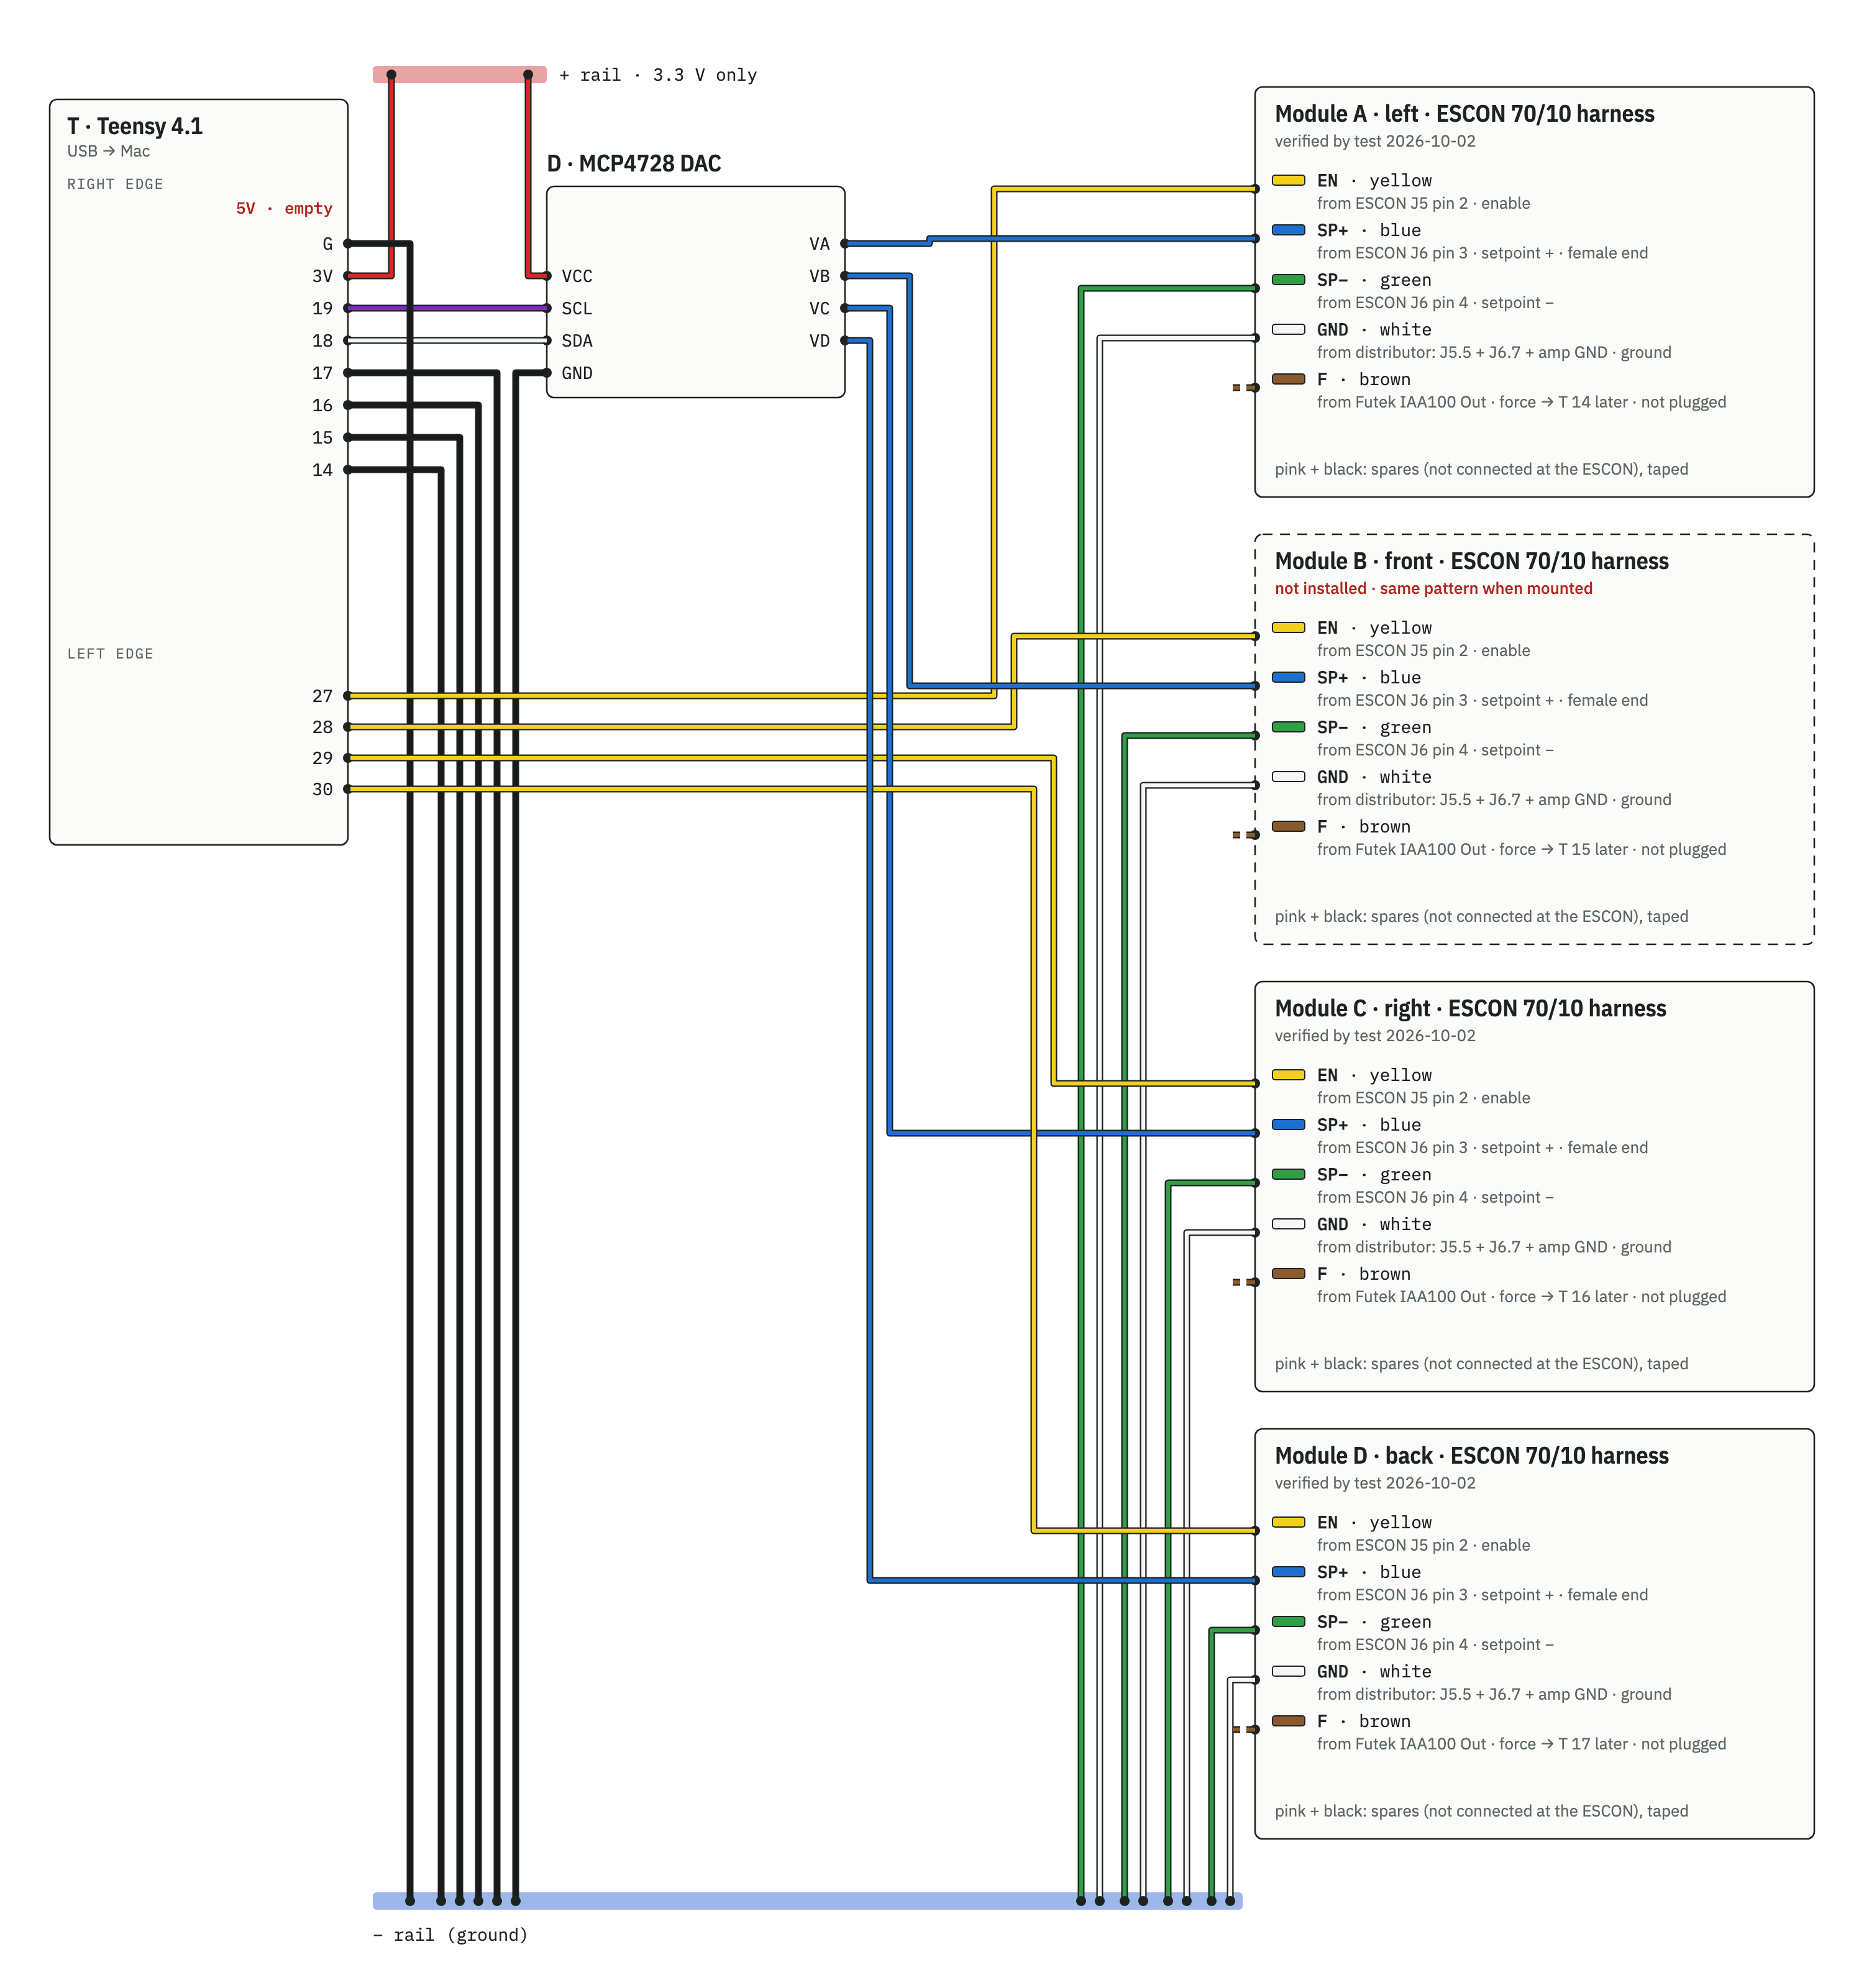
\includegraphics[width=0.78\linewidth]{figures/cabling-4-modules.png}
\caption{Breadboard cabling as of 2 Oct 2026 (\file{docs/diagrams/cabling-4-modules.png}). Since then B is
wired the same way and the brown force wires are plugged in. Valid until the carrier board replaces the
breadboard.}
\end{figure}

\subsection{Carrier PCB}\label{sec:carrier}
The breadboard was the cause of several faults (loose contacts, a wire on the wrong rail). The carrier
board (\file{hardware/carrier/}) holds the Teensy and DAC in sockets and gives each module one pluggable
5-way Phoenix MSTB connector: the module's wires are screwed into its plug once, the plug locks with two
flange screws.

\begin{figure}[H]\centering
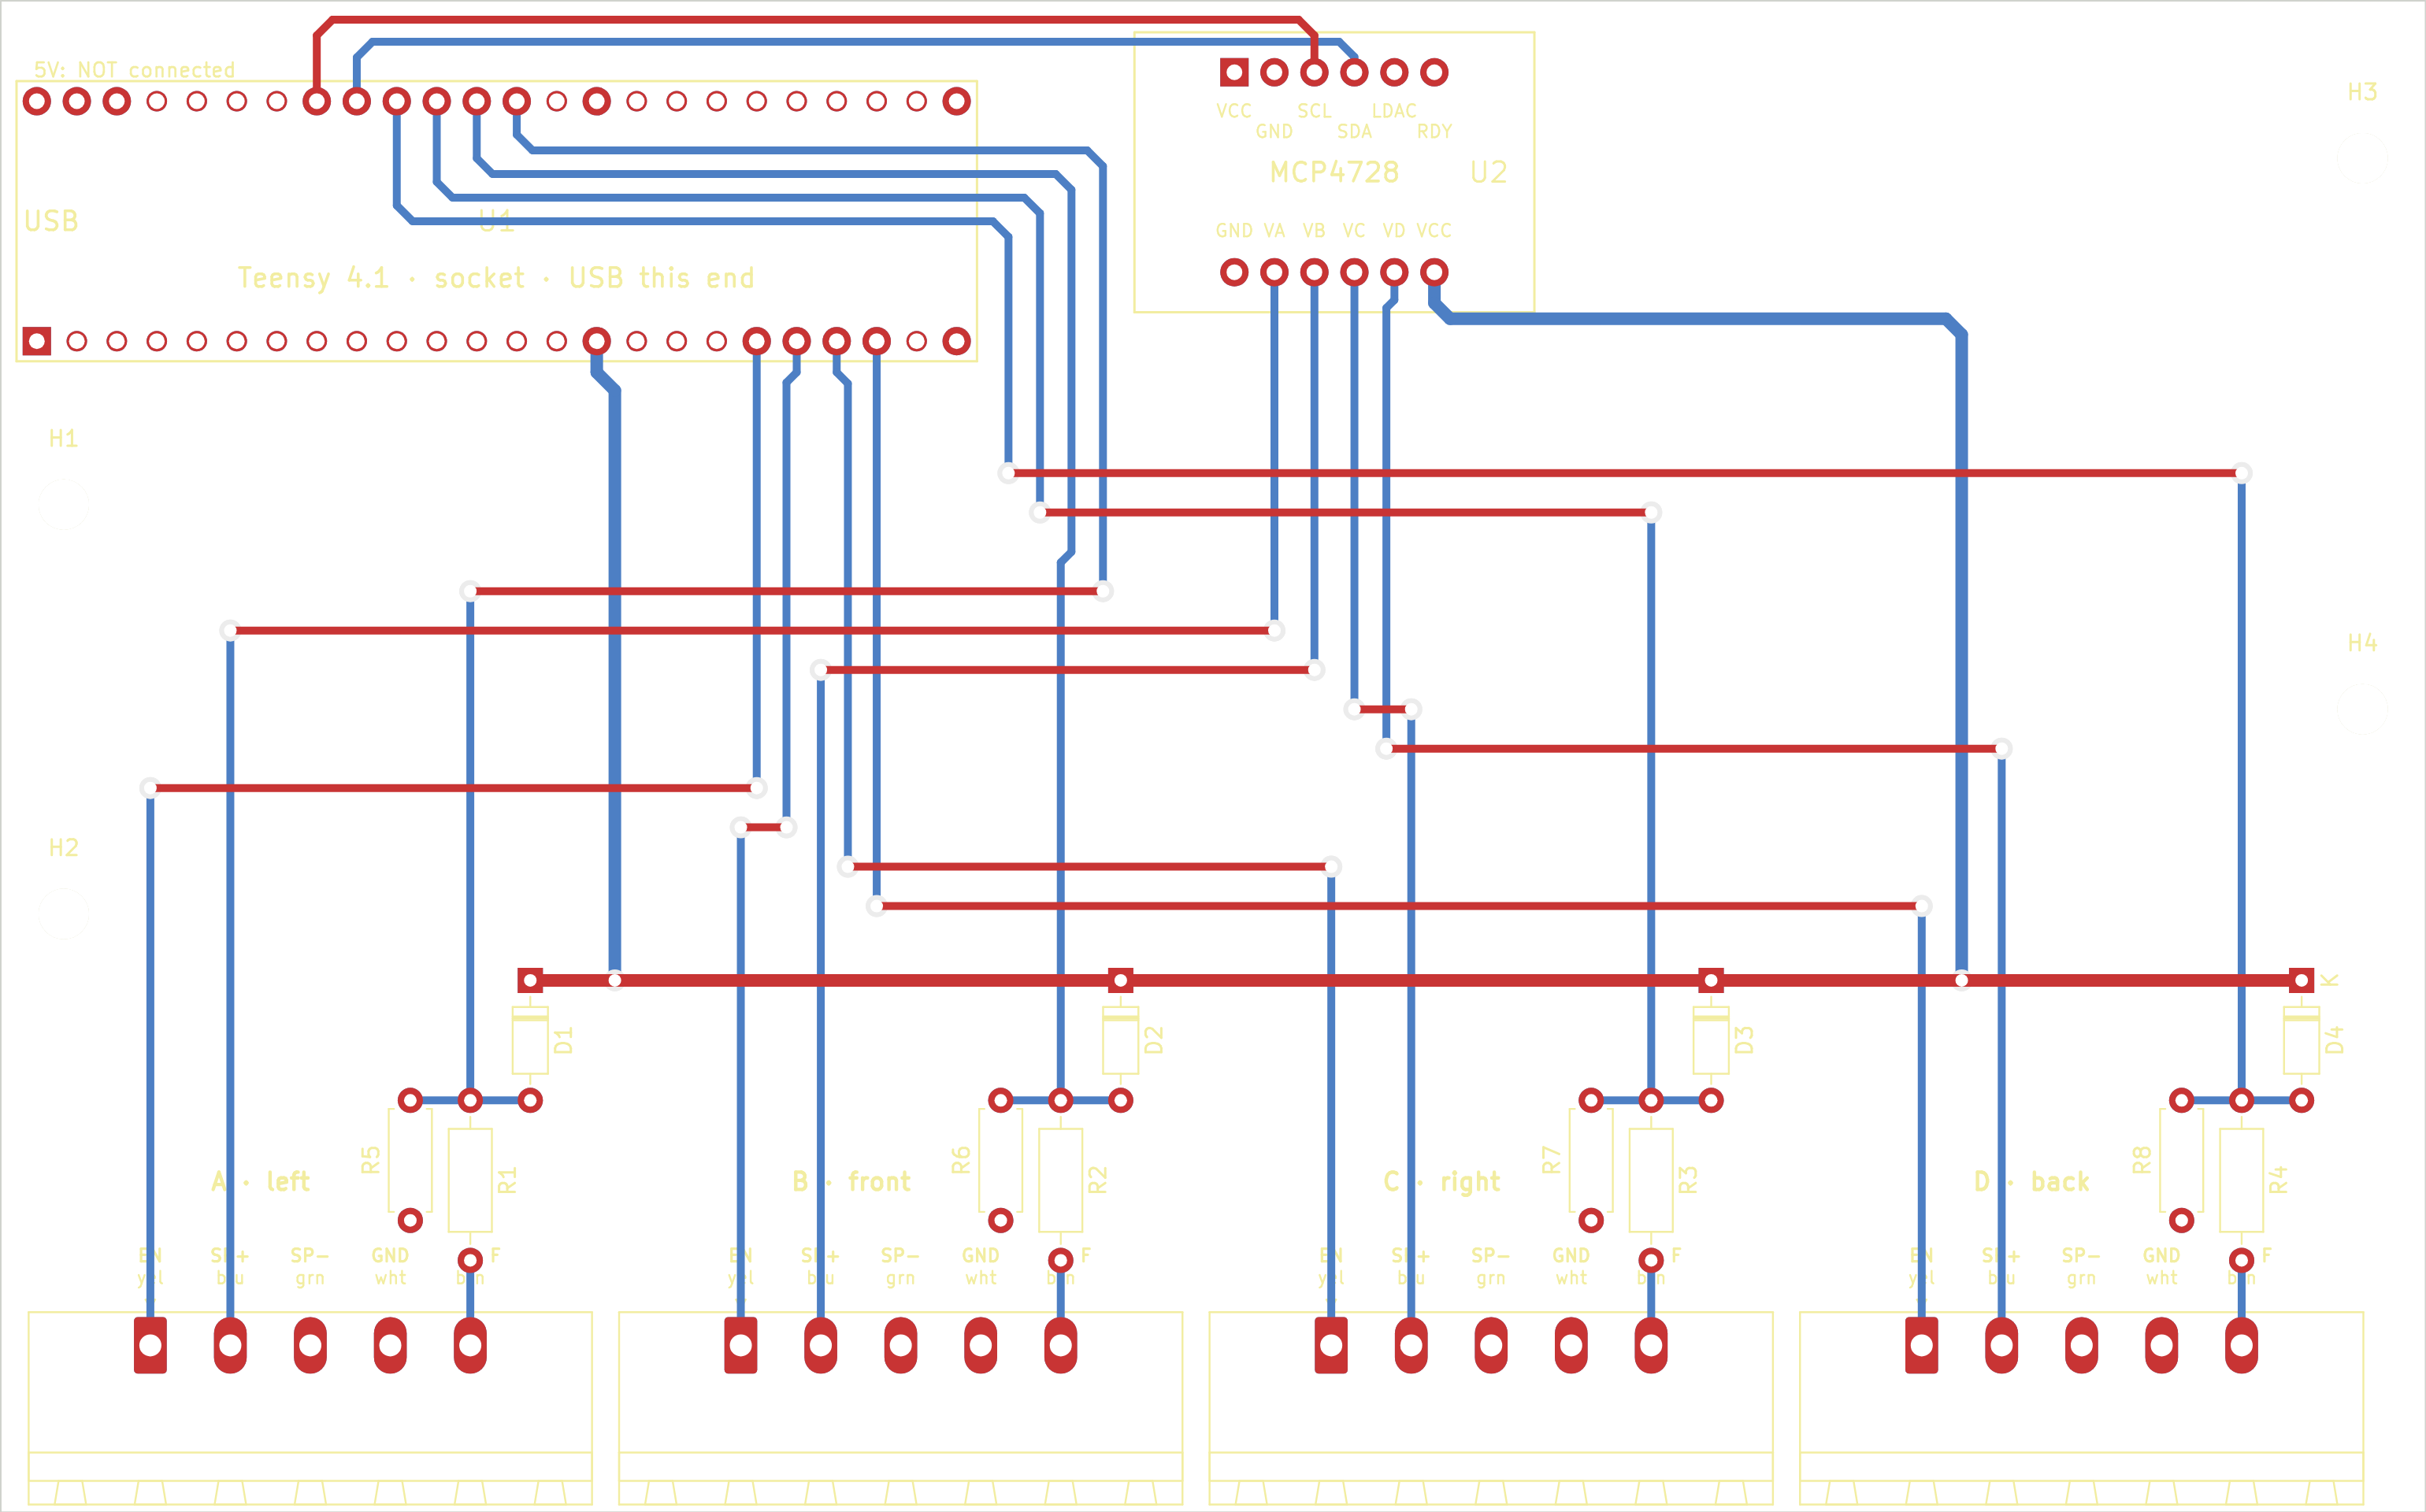
\includegraphics[width=0.85\linewidth]{figures/board-preview.png}
\caption{Carrier board v1, 154$\times$96\,mm, 2 layers, through-hole only. Red: top copper, blue: bottom.
Module plugs J1--J4 (A, B, C, D) at the bottom edge, pins left to right: 1 EN, 2 SP+, 3 SP$-$, 4 GND, 5 F.}
\end{figure}

\paragraph{Force input protection.} Per force input: connector F $\rightarrow$ 1\,k$\Omega$ $\rightarrow$
Teensy pin, 1\,M$\Omega$ to GND, BAT85 diode to 3.3\,V. The Teensy still sees 99.9\,\% of the amplifier
voltage, an unplugged input reads 0\,N, and an amplifier set above 3.3\,V cannot damage the Teensy pin. If an
amplifier can only be set to 0--10\,V, change the pair to a divider (e.g.\ 22\,k$\Omega$ / 10\,k$\Omega$) and
recalibrate.

\paragraph{Changing the board.} Never edit the KiCad files by hand; they are generated. Connections and
values: \file{netlist.py}; placement and routing: \file{gen_carrier.py}; schematic: \file{gen_schematic.py}.
Run \cmd{./build.sh} (KiCad 8): it must report 0 ERC, 0 DRC and 0 parity violations, and it rewrites the
gerber zip and PDFs in \file{fab/}.

\begin{figure}[H]\centering
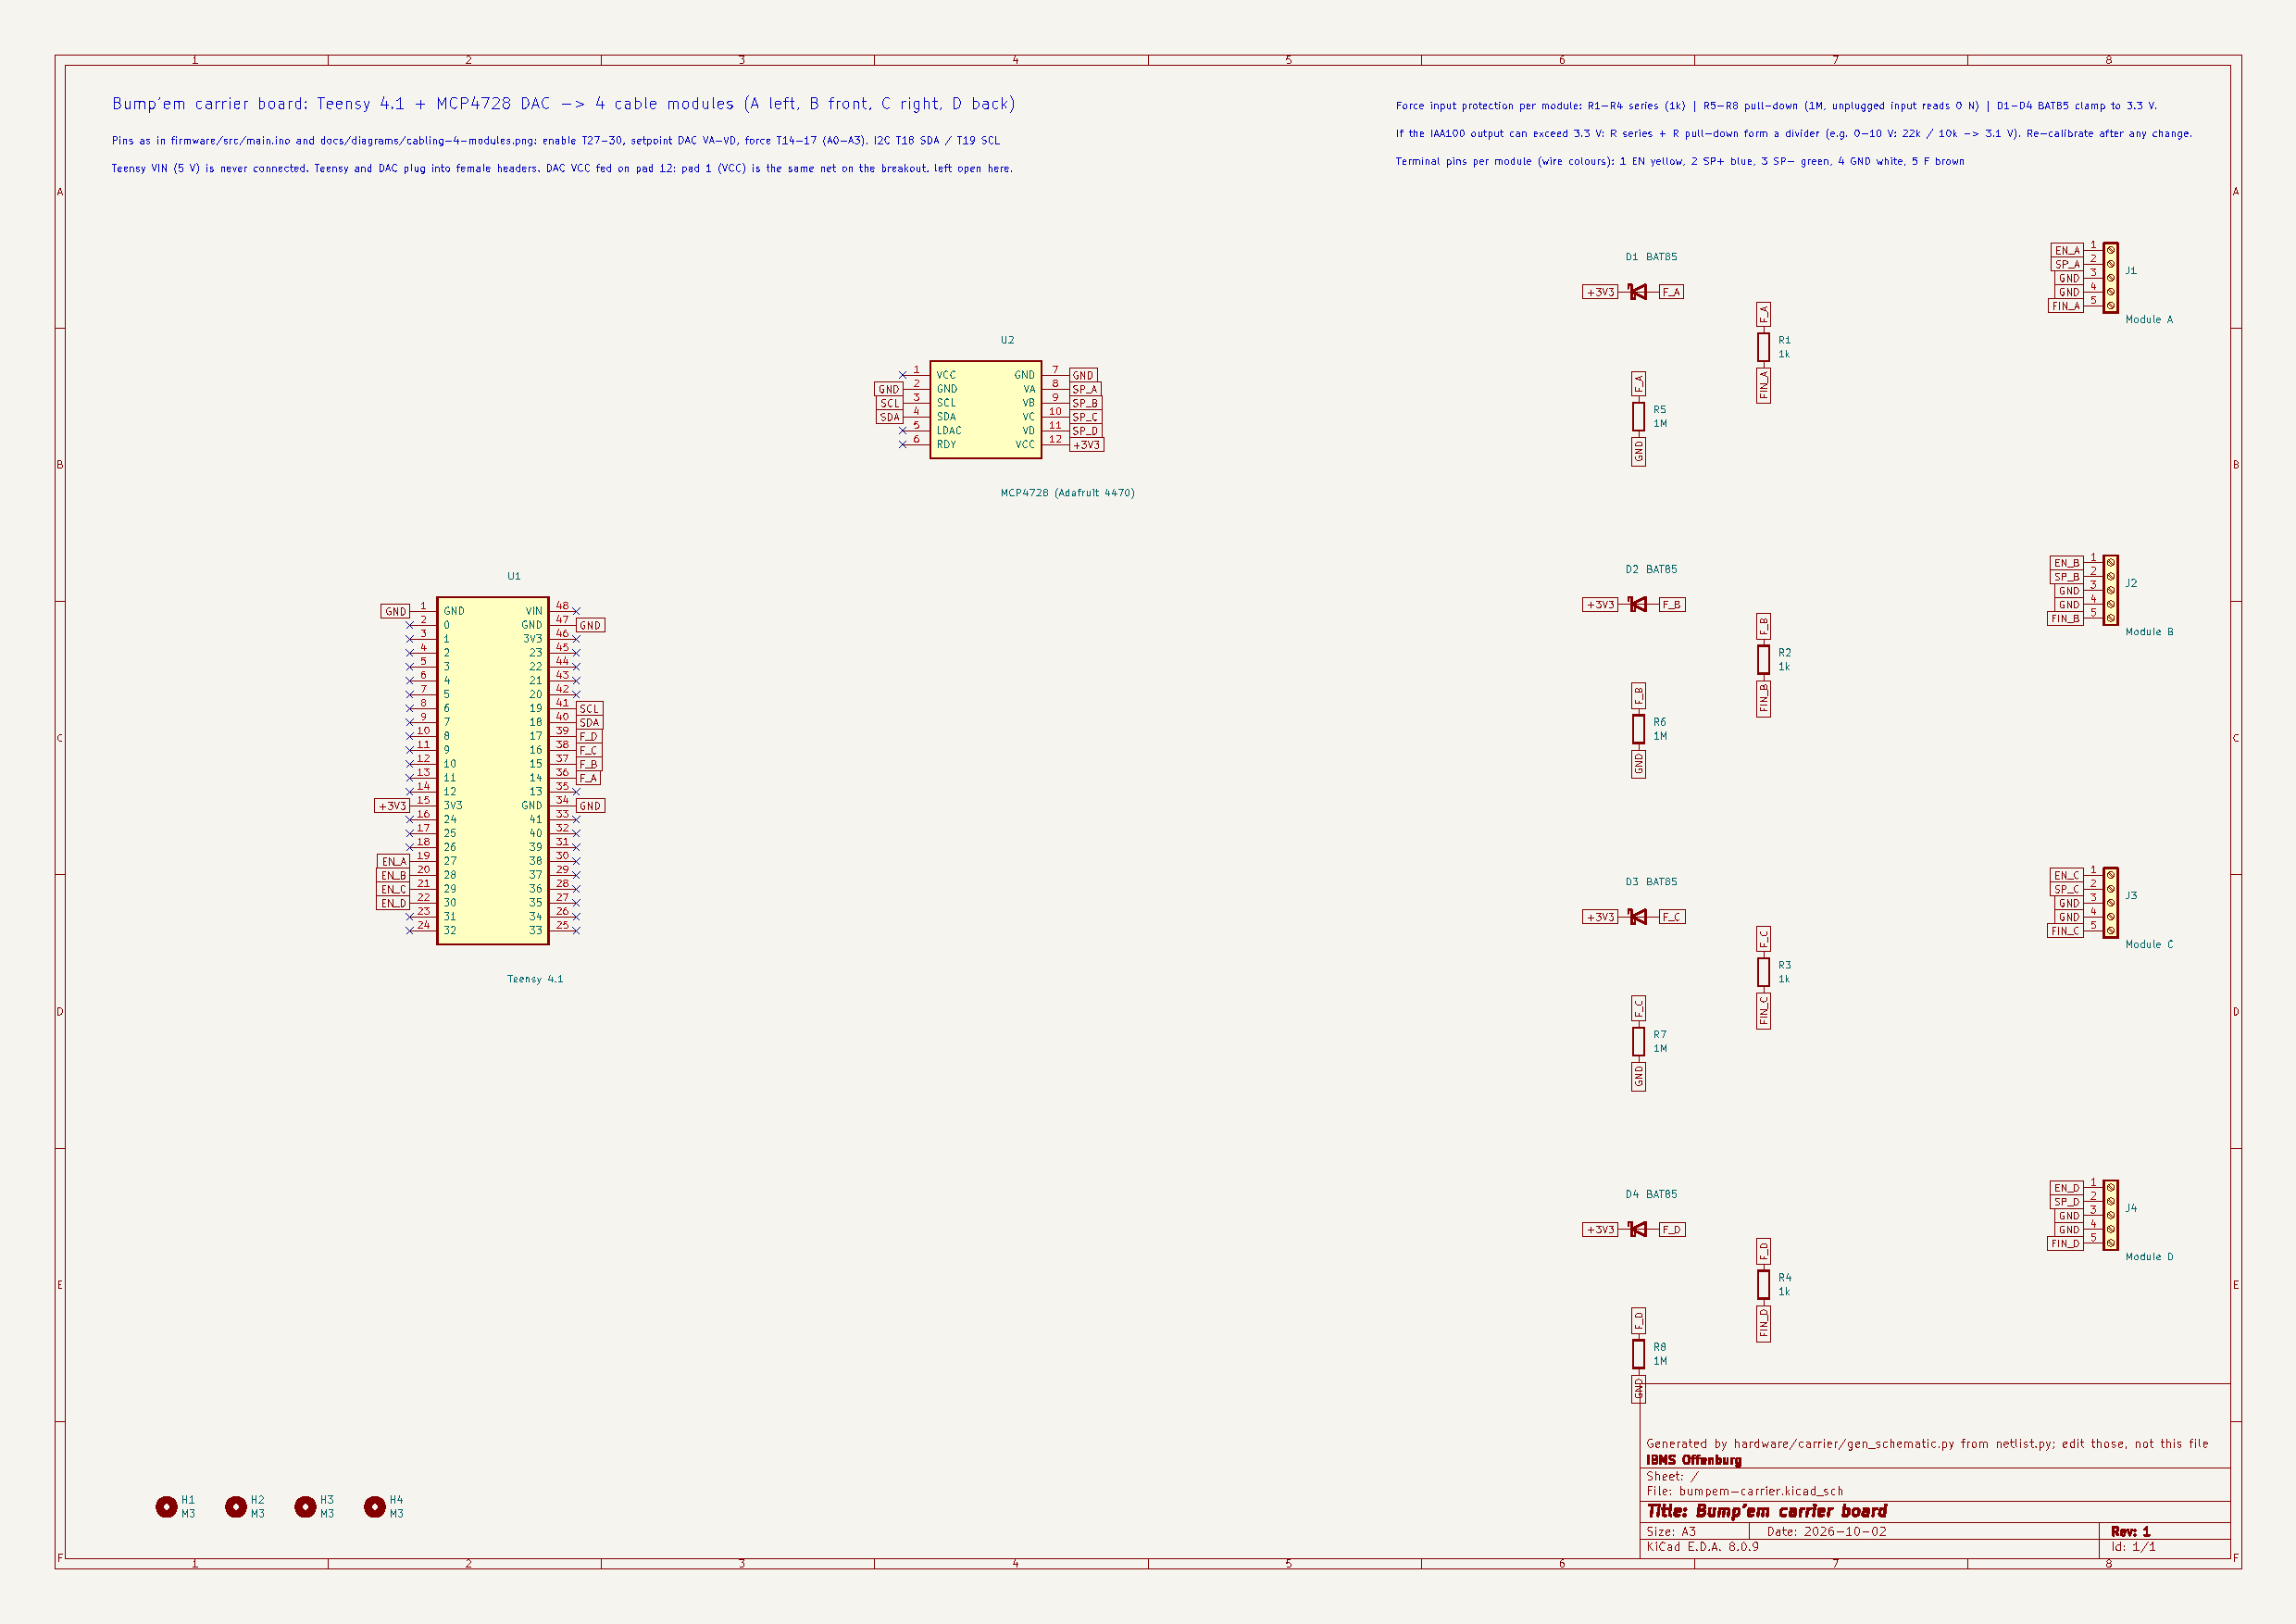
\includegraphics[width=\linewidth]{figures/carrier-schematic.pdf}
\caption{Carrier board schematic (\file{hardware/carrier/fab/bumpem-carrier-schematic.pdf}).}
\end{figure}

\subsection{E-stop (to be wired)}\label{sec:estop}
Stanford's e-stop switches off the 48\,V output of each RSP-2000 through its control connector CN501
(Hirose DF11-12DP):
\begin{itemize}
\item One button with one \textbf{normally open} contact block per 48\,V supply (four towers = four NO blocks
on one button, each pair of wires kept separate).
\item Per supply, two 24\,AWG wires from the contact to CN501 \textbf{pin 7} (Remote ON-OFF) and
\textbf{pin 11} (+5V-AUX). Shorted = 48\,V off.
\item Mating part: DF11-12DS housing with DF11 crimp terminals (or solder, as Stanford did).
\end{itemize}
\warn{This e-stop is not fail-safe: a cut wire means the button does nothing. Test it before every
session (48\,V on, press: every ESCON LED off; release: back on). Ask the technician about a fail-safe
variant. The mains and the supply's auxiliary outputs stay live when it is pressed.}
